\documentclass[conference, letterpaper]{IEEEtran}

\usepackage{booktabs, multicol, makecell, amsmath, adjustbox}
\usepackage{graphicx, tikz,tabularx}
\usepackage{subcaption}
\usetikzlibrary{shapes.geometric, matrix,arrows,positioning,calc,intersections}

% correct bad hyphenation here
\hyphenation{op-tical net-works semi-conduc-tor}

%\usepackage{subcaption}

% *** GRAPHICS RELATED PACKAGES ***
%
%
\usepackage{fancyhdr}

\renewcommand{\thispagestyle}[2]{} 


\fancypagestyle{plain}{
        \fancyhead{}
        \fancyhead[C]{first page center header}
        \fancyfoot{}
        \fancyfoot[C]{first page center footer}
}
\pagestyle{fancy}


\headheight 20pt
\footskip 20pt

\rhead{}

%Enter the first page number of your paper below
\setcounter{page}{1}

%Header
\fancyhead[R]{\textit{(IJACSA) International Journal of Advanced Computer Science and Applications, \\ Vol. XXX, No. XXX, 2014}}
\renewcommand{\headrulewidth}{0pt}

%Footer
\fancyfoot[C]{www.ijacsa.thesai.org}
\renewcommand{\footrulewidth}{0.5pt}
\fancyfoot[R]{\thepage \  $|$ P a g e }


\begin{document}

%
% paper title
% can use linebreaks \\ within to get better formatting as desired
\title{Optimum design of laminated composites for minimum thickness by a variant
of genetic algorithm}


\author{\IEEEauthorblockN{$\text{Huiyao Zhang}^1, \text{ Atsushi Yokoyama}^2$}\\
\IEEEauthorblockA{
Department of Fiber Science and Engineering\\
Kyoto Institute of Technology,\\
Kyoto, JAPAN \\
email:yokoyama@kit.ac.jp \\
}}
% affiliations
% conference papers do not typically use \thanks and this command
% is locked out in conference mode. If really needed, such as for
% the acknowledgment of grants, issue a \IEEEoverridecommandlockouts
% after \documentclass



% make the title area
\maketitle



\begin{abstract}
	The main challenge presented by the laminate composite design is the laminate
layup, involving a set of fiber orientations, composite material systems, and
stacking sequences. In nature, it is a combinatorial optimization problem that
can be solved by the genetic algorithm (GA). In this present study, a new
variant of the GA is proposed for the optimal design by modifying the selection
strategy.  To check the feasibility of a laminate subject to in-plane loading,
the effect of the fiber orientation angles and material components on the first
ply failure is studied. Then we compare the experiment results with works in
other literature.

\end{abstract}

\begin{IEEEkeywords}
Genetic algorithm; Optimization; Classic lamination theory; Failure theory
\end{IEEEkeywords}


% For peer review papers, you can put extra information on the cover
% page as needed:
% \ifCLASSOPTIONpeerreview
% \begin{center} \bfseries EDICS Category: 3-BBND \end{center}
% \fi
%
% For peerreview papers, this IEEEtran command inserts a page break and
% creates the second title. It will be ignored for other modes.
\IEEEpeerreviewmaketitle

\section{Introduction}
Composite materials offer improved strength, stiffness, corrosion resistance,
etc. over conventional materials, and are widely used as alternative materials
for applications in various industries ranging from electronic packaging to golf
clubs, and medical equipment to homebuilding, making aircraft structure to space
vechicles. The stacking sequence and fiber orientation of composite laminates
give the designer additional 'degree of freedom' to tailor the design with
respect to strength or stiffness.  One widely known advange of using composite
material is can significantly reducing the weight of target structure, and many
researchers attempted to improve the efficiency of using composite materail by
mimimizing the thickness\cite { schmit1973optimum, schmit1977optimum,
	fukunaga1991strength, soares1995discrete, le1995improved,
	jayatheertha1996application, wang1996optimum, adali1997minimum,
	correia1997higher, scares1997optimization, abu1998optimum, lombardi1998anti,
	le1998design, sivakumar1998optimum, barakat1999use, richard2000reliability,
moita2000sensitivity, soremekun2001composite, walker2003technique,
di2003multiconstrained, kere2003using}.

In practice, fiber orientations are restricted to a finite set of angles, and
ply thickness is a specific numberic value.  Because the design variables are
not continueous, a gradient based optimization procedure, such as gradient
descent method, is not suitable to cope with such problems.  Moreover, gradient
based optimization approach is very eazily to get trapped in local minima, and
many local optimum may exist in structural optimization problems. A stochastic
optimization, such as genetic algorithm(GA) and simulated annealing(SA), is able
to deal with optimization problem with discrete variables. Besides, stochastic
method could escape from local optimum, and obtain global optimum.  GA is one of
the most reliably stochastic algorithm, which has been widely used in solving
constraint desgin for composite
laminate\cite{callahan1992optimum,soremekun2001composite,park2001stacking,walker2003technique,deka2005multiobjective,pelletier2006multi,jadhav2007parametric,kim2007development,park2008improved}.
Although GA gains different advantages for solving discrete problems, many
disadvantages exists within this approach. First, the optimization process of GA
parameters, such as the population size, parent population,mutation percentage,
etc., is very tedious; Second, the GA needs to evaluate the objective functions
many times to acheive the optimization, and the compuation cost is very high;
the last problem within GA is the premature convergence. GA consists of five
basic parts: the variable coding, selection scheme, crossover operator, mutation
operator and how the constraints are handled.

The first issue when implementing a GA is the representation of design
variables, and an appropriate design representation is crucial to enhance the
efficiency of GA. The canonical GA has always used binary strings to encode
alternative solutions, however, some argued that the minimal cardinality, i.e.,
the binary representation, are not the best option. Real value string has been
widely employed in 

Selection scheme plays a critical role in balancing the dilemma of exploration
and exploitation inherented in GA, and various selection methods, for example,
roulette wheel, elitist, and tournament etc., have been proposed to overcome
this issue. Both of roulette selection and tournament selection are well-studied
and widely employed in the optimization design of laminated composite due to
their simplicity to code and efficiency for both nonparallel and parallel
architectures.

Crossover is another crucial operator introduced into the GA
methodology framework, in which the alternative solution is generated from the
mating pool.  multiple types of crossover operator has been utilized in the optimization
design of composite structures, such as: one-point, two-point, and uniform
crossover.


GA is originally proposed for unconstrained optimization. However, in order to
deal with constrained design for composite laminate, some techiques were
introduced into the GA. The first method is using of data structure, special
data structure was developed to fulfils the symmetry constraint of the laminate,
which consists of coding only half of the laminate and considering that each
stack of the laminate is formed by two laminae with the same orientation but
opposite signs\cite{le1995improved,kogiso1994design}. A penalty function is
developed to convert a constrained problem into an unconstrained problem by
adding penalty term to the objective funtion. Another method to solve
constrained problem is introducing repair strategy by Todoroki and Haftka
\cite{todoroki1998stacking}, which is aim to transform infeasible solutions to
feasible solution by incorporating problem-specific knowledge. 

Another major concern within GA is the convergence speed in terms of the time
and computation cost needed to reach a solution of desired quality. The
objective function based on the CLT is excessively time-consuming and complicate
to evaluate, in addition, the target function of GA  needs to be calculate many
times. The traditional method to deal with this issue is by increasing the
selection pressure to accelerate the convergence speed, however, in some cases,
this approach does not acheive an ideal result. Becasue the GAs just provides a
methodological framework to deal with trickey problems, which is heavily
inspired by evolution of biology, it is unnecessary to exactly follow all the
GA operation. It is possible to just perform one or more GA operations, and
incorporate other techiques into GA. In present study, a variant of mutation
operator is introduced to accelerate the convergence process.
  

To check the feasibility of a laminate composite by imposing a strength
constraint, various failure criterion have been proposed to decide whether it
fails or not, such as  maximum stress failure theory, maximum strain failure
theory, Tsai-Hill Failure theory and Tsai-Wu criterion. Each theory is proposed
based on massive experiment data or complicate mathematical model, however
single use any of them may lead to false optimum design for some loading case
due to the particular shape of its failure envelope. In order to overcome this
disadvantage within every failure theory, two reliably failure criteria, maximum
stress theory and Tsai-wu criterion are employed to check whether the composite
laminate fullfils the constraint.


The rest of the paper is organized as follows. Section 2 explains the classical laminate theory and
the failure criteria taken in the present study.  Section 3 explains the proposed method of
selection strategy and self-adaptative parameters for mutation during the GA process. Section 4
describes the result of the numerical experiments in different cases, and in the Conclusion section
we dicuss the results.







\section{Introduction}
Fiber-reinforced composite materials have been widely used in many industries
because they offer improved mechanical stiffness, strength, and low specific
gravity of fibers  over conventional materials. The use of composite material
materials in structural application is range from electronic packaging, sports
equipment, homebuilding, medical prosthetic devices, to high performance
military structures. The stacking sequence, ply thickness, and fiber
orientation of composite laminates give the designer additional ’degree of
freedom’ to tailor the design with respect to strength or stiffness. Classic
lamination theory(CLT) is taken to predict the behavior of a laminate from a
knowledge of the composite laminate properties of the individual layers and the
laminate geometry.

Evolutionary artificial neural networks(EANN's) is a special class of artifical
neural networks(ANN's) in which evolutionary algorithms(ES's) are introduced to
learn the optimal ANN. EA's can be used in the ANN at three different levels:
connection weights, architectures, input features, and learning rules. It is
shown, the combinations of ANN's and EA's can significantly improve the
performance of intelligent systems that rely's on ANN's or EA's alone.



The rest of the paper is organized as follows. Section 2 explains the classical
laminate theory and the failure criteria taken in the present study. Section 3
explains the design of artifical neural network for mathmatical model
approximation.  Section 4 reviews the use of genetic algorithm in the design of
neural network architecture and the parameters optimization during the training
process of neural network.  design Section 4 describes the result of the
numerical experiments in different cases, and in the Conclusion section we
dicuss the results.
\section{Classic Lamination Theory}
Classical lamination theory is based upon three simplifying engineering
assumptions: (1) Each layer's thickness is very small and consist of
homogeneous, orthotropic material, and these layers are prefectly bonded
together; (2) The entire laminated composite is supposed to be under plane
stress; (3) Normal cross sections of the entire laminate is normal to the
deflected middle surface, and do not change in thickness.
\begin{figure}
\centering
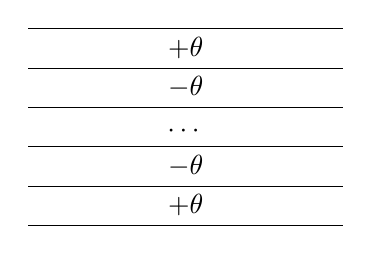
\begin{tikzpicture}
	\draw (0,0) -- (4,0);
	\draw (0,-0.5) -- (4,-0.5) node[midway, above] {$\mathit{+}\theta$};
	\draw (0,-1) -- (4,-1) node[midway, above] {$\mathit{-}\theta$} ;
	\draw (0,-1.5) -- (4,-1.5) node[midway, above] {$\cdots$};
	\draw (0,-2) -- (4,-2) node[midway, above] {$\mathit{-}\theta$};
	\draw (0,-2.5) -- (4,-2.5) node[midway, above] {$\mathit{+}\theta$};
\end{tikzpicture}
\caption{Model for Angle ply laminate}
\end{figure}

\subsection{Stress and Strain in a Lamina}
For a single lamina has a small thickness under plane stress, and it's upper and lower surfaces of the lamina are
free from external loads. According to the Hooke's Law, the three-dimensional stress-strain equations can be reduced to
two-dimensional stress-strain equations. The stress-strain relation in local axis 1-2 is:
\begin{equation}
    \begin{bmatrix}
        \sigma _1\\
        \sigma _2\\
        \tau_{12}
    \end{bmatrix}
    =
    \begin{bmatrix}
        Q_{11} & Q_{12} & 0\\
        Q_{12} & Q_{22} & 0\\
        0      &  0     & Q_{66}
    \end{bmatrix}
    \begin{bmatrix}
        \varepsilon_1\\
        \varepsilon_2\\\gamma_{12}
    \end{bmatrix}
\end{equation}
where $Q_{ij} $are the stiffnesses of the lamina that are related

to engineering elastic constants given by
\begin{equation}
    \begin{split}
    &Q_{11}=\frac{E_1}{1-v_{12}v_{21}}\\
    &Q_{22}=\frac{E_2}{1-v_{12}v_{21}}\\
    &Q_{66}=G_{12}\\
    &Q_{12}=\frac{v_{21}E_2}{1-v_{12}v_{21}}\\
    \end{split}
\end{equation}

where $E_1, E_2, v_{12}, G_{12} $ are four independent engineering elastic constants, which are defined as follows: $E_1 $ is the longitudinal Young's modulus, $E_2 $ is the transverse Young's modulus, $v_{12} $ is the major Poisson's ratio, and $G_{12} $ is the in-plane shear modulus.

Stress strain relation in the global x-y axis:
\begin{equation}
	\label{equ:stress-strain}
	\left[\begin{array}{l}
			\sigma _{x} \\ \sigma _{y} \\
			\tau_{xy}\end{array}\right]=\left[\begin{array}{lll}\bar{Q}_{11} &
			\bar{Q}_{12} & \bar{Q}_{16}\\ 
			\bar{Q}_{12} & \bar{Q}_{22} & \bar{Q}_{26} \\
								\bar{Q}_{16} & \bar{Q}_{26}
			 &\bar{Q}_{66}\end{array}\right]\left[\begin{array}{l}\varepsilon_{x}
	 \\ \varepsilon_{y}\\ \gamma_{x y}\end{array}\right] \end{equation}
where
\begin{equation}
	\begin{array}{l}
		\resizebox{.35\textwidth}{!}{$\bar{Q}_{11}=Q_{11} cos^{4}\theta+Q_{22} sin^{4}\theta+2\left(Q_{12}+2
		Q_{66}\right) sin^{2}\theta cos^{2}\theta$} \\

		\resizebox{.35\textwidth}{!}{$\bar{Q}_{12}=\left(Q_{11}+Q_{22}-4 Q_{66}\right) sin^{2}\theta
		cos^{2}\theta+Q_{12}\left(cos^{4}\theta+sin^{2}\theta \right)$} \\

		\resizebox{.35\textwidth}{!}{$\bar{Q}_{22}=Q_{11} sin^{4}\theta+Q_{22} cos^{4}\theta+2\left(Q_{12}+2
		Q_{66}\right) sin^{2}\theta cos^{2}\theta$} \\

		\resizebox{.4\textwidth}{!}{$\bar{Q}_{16}=\left(Q_{11}-Q_{12}-2
		Q_{66}\right) cos^{3}\theta sin\theta-\left(Q_{22}-Q_{12}-2Q_{66}\right)
	sin^{3}\theta cos\theta$} \\ 
		\resizebox{.4\textwidth}{!}{$\bar{Q}_{26}=\left(Q_{11}-Q_{12}-2
		Q_{66}\right) cos\theta sin^{3}\theta-\left(Q_{22}-Q_{12}-2
Q_{66}\right)cos^{3}\theta sin\theta$}
		 \\ 
	\resizebox{.4\textwidth}{!}	{$\bar{Q}_{66}=\left(Q_{11}+Q_{22}-2 Q_{12}-2 Q_{66}\right)
	sin\theta^{2}cos\theta^{2}+Q_{66}\left(sin\theta^{4}+cos\theta^{4}\right)$}\\
	\end{array}
\end{equation}



The local and global stresses in an angle lamina are related

to each other through the angle of the lamina $\theta $
\begin{equation}\left[\begin{array}{l}\sigma _{1} \\ \sigma _{2} \\ \tau_{12}\end{array}\right]=[T]\left[\begin{array}{l}\sigma _{x} \\ \sigma _{y} \\\tau_{xy}\end{array}\right]
\end{equation}

where
\begin{equation}
	[T]=\left[\begin{array}{ccc}cos^{2}\theta & sin^{2}\theta & 2
		sin\theta cos\theta \\ 
sin^{2}\theta & cos^{2}\theta & -2 sin\theta cos\theta \\
-sin\theta cos\theta
			  & sin\theta cos\theta  &cos^{2}\theta -sin^{2}\theta
\end{array}\right] 
\end{equation}



\subsection{Stress and Strain in a Laminate}
For forces and moment resultants acting on laminates, such as in plate and shell
structures, the relationship between applied forces and moment and displacement
can be given by

\begin{equation} \label{eq:force_and_moments}
	\begin{array}{l}
		\begin{aligned}
	\begin{bmatrix}
		N_x \\
		N_y \\
		N_{xy}
	\end{bmatrix}
	&=
	\begin{bmatrix}
		A_{11} & A_{12} & A_{16} \\
		A_{12} & A_{22} & A_{26} \\
		A_{16} & A_{26} & A_{66} 
	\end{bmatrix}
    \begin{bmatrix}
		\varepsilon_x^0 \\
        \varepsilon_y^0 \\
		\gamma_{xy}^0
    \end{bmatrix}   \\
	&+               
	\begin{bmatrix}
		B_{11} & B_{12} & B_{16} \\
		B_{11} & B_{12} & B_{16} \\
		B_{16} & B_{26} & B_{66} 
	\end{bmatrix}
	\begin{bmatrix}
		k_x \\
		k_y \\
		k_{xy} 
	\end{bmatrix}  \\
\end{aligned} \\ \\
\begin{aligned}
	\begin{bmatrix}
		M_x \\
		M_y \\
		M_{xy}
	\end{bmatrix}
	&=
	\begin{bmatrix}
		B_{11} & B_{12} & B_{16} \\
		B_{12} & B_{22} & B_{26} \\
		B_{16} & B_{26} & B_{66} 
	\end{bmatrix}
    \begin{bmatrix}
		\varepsilon_x^0 \\
        \varepsilon_y^0 \\
		\gamma_{xy}^0
    \end{bmatrix} \\ 
	&+  
	\begin{bmatrix}
		D_{11} & D_{12} & D_{16} \\
		D_{11} & D_{12} & D_{16} \\
		D_{16} & D_{26} & D_{66} 
	\end{bmatrix}
	\begin{bmatrix}
		k_x \\
		k_y \\
		k_{xy} 
	\end{bmatrix}
\end{aligned}
	\end{array}
\end{equation}


$N_x,N_y $  - normal force per unit length

$N_{xy} $  - shear force per unit length

$M_x, M_y $ - bending moment per unit length

$M_{xy} $  - twisting moments per unit length

$\varepsilon^{0}, k $- mid plane strains and curvature of a laminate in x-y coordinates

The mid plane strain and curvature is given by
\begin{equation}
    \begin{split}
    &A_{ij}=\sum_{k=1}^{n}(\overline{Q_{ij}})_k(h_k-h_{k-1})  i=1,2,6, j=1,2,6\\
    &B_{ij}=\frac{1}{2}\sum_{k=1}^{n}(\overline{Q_{ij}})_k(h_k^2 - h_{k-1}^2)  i=1,2,6, j=1,2,6\\
    &D_{ij}=\frac{1}{3}\sum_{k=1}^{n}(\overline{Q_{ij}})_k(h_k^3 - h_{k-1}^3) i=1,2,6, j=1,2,6\\
    \end{split}
\end{equation}

The [A], [B], and [D] matrices are called the extensional, coupling, and bending stiffness matrices,
respectively. The extensional stiffness matrix $[A]$ relates the resultant in-plane forces to the
in-plain strains, and the bending stiffness matrix $[D]$ couples the resultant bending moments to
the plane curvatures.  The coupling stiffness matrix $[B]$ relates the force and moment terms to the
midplain strains and midplane curvatures.

\section{Failure criteria for a lamina}

Failure criteria for composite materials are more difficult to predict due to
structural and material complexity in comparison to isotropic materials. The
failure process of a composite materials can be regarded from microscopic and
macroscopic points of view. Most popular criteria about the failure of an angle
lamina are in terms of macroscopic failure criteria, which are based on the
tensile, compressive and shear strengths. According to the failure surfaces,
these criteria
\cite{massard1984computer,reddy1987first,fang1993design,soeiro1994multilevel,pelletier2006multi,jadhav2007parametric,omkar2008artificial,choudhury2019failure},
can be classified into two classes: one is called independent failure mode
criteria which includes the maximum stress failure
theory\cite{watkins1987multicriteria}, maximum strain failure theory because
their failure envelop are rectangle; another is called quadratic polynomial
which includes Tsai-Wu\cite{martin1987optimum,soares1995discrete}, Chamis,
Hoffman and Hill criteria because their failure surfaces are of ellipsoidal
shape. In the present study, two most reliable failure criteria is taken,
Maximum stress and Tsai-wu.  Both of these two failure criteria are based on
the stresses in the local axes instead of principal normal stresses and maximum
shear stresses, and four normal strength parameters and one shear stress for a
unidirectional lamina are involved. The five strength parameters are

$(\sigma _1^{T})_{ult}= $ ultimate longitudinal tensile strength(in direction 1),

$(\sigma _1^{C})_{ult}= $ ultimate longitudinal compressive strength,

$(\sigma _2^{T})_{ult}= $ ultimate transverse tensile strength,

$(\sigma _2^{C})_{ult}= $ ultimate transverse compressive strength, and

$(\tau_{12})_{ult}= $ and ultimate in-plane shear strength.

\begin{figure}
\centering
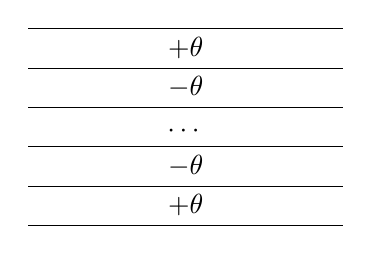
\begin{tikzpicture}
	\draw (0,0) -- (4,0);
	\draw (0,-0.5) -- (4,-0.5) node[midway, above] {$\mathit{+}\theta$};
	\draw (0,-1) -- (4,-1) node[midway, above] {$\mathit{-}\theta$} ;
	\draw (0,-1.5) -- (4,-1.5) node[midway, above] {$\cdots$};
	\draw (0,-2) -- (4,-2) node[midway, above] {$\mathit{-}\theta$};
	\draw (0,-2.5) -- (4,-2.5) node[midway, above] {$\mathit{+}\theta$};
\end{tikzpicture}
\caption{Model for Angle ply laminate}
\end{figure}


\subsection{Maximum stress failure criterion}(MS)


Maximum stress failure theory consists of maximum normal stress theory proposed by Rankine and maximum 
shearing stress theory by Tresca. The stresses applied on a lamina can be resolved into the normal and shear stresses 
in the local axes. If any of the normal or shear stresses in the local axes of a lamina is equal or exceeds the corresponding 
ultimate strengths of the unidirectional lamina, the lamina is considered to be failed. That is,

$\sigma_1 \geq (\sigma _1^{T})_{ult} $ or $\sigma_1 \leq -(\sigma _1^{C})_{ult} $

$\sigma_2 \geq (\sigma _2^{T})_{ult} $ or $\sigma_2 \leq -(\sigma _2^{C})_{ult} $

$\tau_{12} \geq (\tau_{12})_{ult} $  or $\tau_{12} \leq -(\tau_{12})_{ult} $

where $\sigma_1$ and $\sigma_2$ are the normal stresses in the local axes 1 and 2, respectively;
$\tau_{12}$ is the shear stress in the symmetry plane 1-2.

\subsection{Tsai-wu failure criterion}
The TW criterion is one of the most reliable static failure criteria which is derived from the von
Mises yield criterion.  
A lamina is considered to fail
if \begin{equation} \label{eq:tsai_wu}
\begin{split}
	H_1 \sigma_1  & + H_2 \sigma_2 + H_6 \tau_{12} + H_{11}\sigma_1^2 + H_{22} \sigma_2^2 \\
				  & + H_{66}  \tau_{12}^2 + 2H_{12}\sigma_1\sigma_2 < 1
\end{split}
\end{equation}

is violated, where

\begin{equation}
	\begin{split}
		H_{1}&=\frac{1}{\left(\sigma_{1}^{T}\right)_{u l t}}-\frac{1}{\left(\sigma_{1}^{C}\right)_{u l t}} \\
		H_{11}&=\frac{1}{\left(\sigma_{1}^{T}\right)_{u l t}\left(\sigma_{1}^{C}\right)_{u l t}} \\
		H_{2}&=\frac{1}{\left(\sigma_{2}^{T}\right)_{u l t}}-\frac{1}{\left(\sigma_{2}^{C}\right)_{u l t}} \\
		H_{22}&=\frac{1}{\left(\sigma_{2}^{T}\right)_{u l t}\left(\sigma_{2}^{C}\right)_{u l t}} \\
		H_{66}&=\frac{1}{\left(\tau_{12}\right)_{u l t}^{2}} \\
		H_{12}&=-\frac{1}{2} \sqrt{\frac{1}{\left(\sigma_{1}^{T}\right)_{u l
		t}\left(\sigma_{1}^{C}\right)_{u l t}\left(\sigma_{2}^{T}\right)_{u l
		t}\left(\sigma_{2}^{C}\right)_{u l t}}}
	\end{split}
\end{equation}

$H_i$ is the strength tensors of the second order; $H_{ij}$ is the strength
tensors of the fourth order. $\sigma_1$ is the applied normal stress in 
direction 1; $\sigma_2$ is the applied normal stress in the direction 2; and
$\tau_{12}$ is the applied in-plane shear stress.





\begin{figure}
\centering
\begin{tikzpicture}
	\begin{scope}
		%\draw[style=help lines] (-3,-3) grid (3,3);
		\draw (0,0) rectangle (2,3);
		\draw[->] (1.3,1.2) -- (2.6,1.2);
		\draw[->] (1.3,1.2) -- (1.3,3.4);
		\node at (2.2,1) {$X_T$};
		\node at (1.5, 3.2) {$Y_T$};
		\node at (-0.2, 0.9) {$X_C$};
		\node at (1.8, -0.2) {$Y_C$};
	\end{scope}
	\begin{scope}[xshift=6cm,yshift=1.15cm]
		%\draw[style=help lines] (-3,-3) grid (3,3);
		\draw[rotate=30] (0,0) ellipse (2cm and 1cm);
		\draw[->] (0.2,0) -- (0.2,2.2);
		\draw[->] (0.2,0) -- (1.9,0);
		\node at (1.6,-0.2) {$X_T$};
		\node at (0.3, 1.3) {$Y_T$};
		\node at (-1.6, 0) {$X_C$};
		\node at (-0.5, -1.5) {$Y_C$};
	\end{scope}
\end{tikzpicture}
\caption{Schematic failure surfaces for maximum stress and quadratic failure
criteria}
\end{figure}


\subsection{Failure Theories for a Laminate}
If keep increasing the loading applied to a laminate, the laminate will fails. The failure process
of a laminate is more complicate than a lamina, because a laminate consists of multiple plies, and
the fiber orientation, material, thickness of each ply maybe different from the others. In most
situations, some layer fails first and the remains continue to take more loads until all the plies
fail.  If one ply fails, it means this lamina does not contribute to the load carrying capacity of
the laminate. The procedure for finding the first failure ply given follows the fully discounted
method:

\begin{enumerate}
\item Compute the reduced stiffness matrix [Q] referred to as the local axis for each ply using its
	four engineering elastic constants $E_1 $, $E_2 $, $E_{12} $, and $G_{12} $.

\item Calculate the transformed reduced stiffness $[\bar{Q}] $ referring to the global coordinate
	system (x, y) using the reduced stiffness matrix [Q] obtained in step 1 and the ply angle for
	each layer.

\item  Given the thickness and location of each layer, the three laminate stiffness matrices [A],
	[B], and [D] are determined.

\item  Apply the forces and moments, $[N]_{xy}, [M]_{xy} $ solve Equation
	\ref{eq:force_and_moments}, and calculate the middle plane strain $[\sigma ^{0}]_{xy} $ and
	curvature $[k]_{xy} $.

\item Determine the local strain and stress of each layer under the applied load.

\item  Use the ply-by-ply stresses and strains in the Tsai-wu failure theory to find the strength
	ratio, and the layer with smallest strenght ratio is the first failed ply. 
\end{enumerate}

\subsection{Safety factor}
The safety factor, or yield stress, is how much extra load beyond is intended a
composite laminate will actually take. The safey factor is defined as 

\begin{equation} \label{eq:sr}S R=\frac{\text {Maximum Load Which Can Be Applied}}{\text {Load Applied}}
\end{equation}.

\subsection{Safety factor}
The safety factor, or yield stress, is how much extra load beyond is intended a
composite laminate will actually take, which is an indication of the material's
load carrying capacity. If the value is less then 1.0, it means failure. The safey factor is defined as 

\begin{equation} \label{eq:sr}S R=\frac{\text {Maximum Load Which Can Be Applied}}{\text {Load Applied}}
\end{equation}.

The safety factor based on maximum stress theory is calculated by the following
method: first, the principal stresses($\sigma_1^k$,$\sigma_2^k$, and
$\tau_{12}^k$) are obtained by experiment; evaluate the safety factor along each
direction according to equation \ref{eq:sr}; The minimum value among these
safety factors are denoted as the safety factor of the lamina, $SF_{MS}^k$.

\begin{align}
	SF_{MS}^k = \text{min of}
	\begin{cases}
		SF_X^k = 
		\begin{cases}
			\frac{X_t}{\sigma_{11}}, \text{ if } \sigma_{11}>0 \\
			\frac{X_c}{\sigma_{11}}, \text{ if } \sigma_{11}<0 \\
		\end{cases} \\
		SF_Y^k = 
		\begin{cases}
			\frac{Y_t}{\sigma_{22}}, \text{ if } \sigma_{22}>0 \\
			\frac{Y_c}{\sigma_{22}}, \text{ if } \sigma_{22}<0 \\
		\end{cases} \\
		SF_S^k =
		\begin{cases}
			\frac{S}{|\tau_{12}|} \\
		\end{cases} \\
	\end{cases}
\end{align}


Assuming the composite laminate under a in-plane loading f, the corresponding
stress on local stress in direction 1, local stress in direction 2, and shear
stress for the kth lamina are $\sigma_1 SF_{TW}^k$, $\sigma_2SF_{TW}^k$, and $\tau_{12}SF_{TW}^k$,
respectively. Substitute them into the equation \ref{eq:tsai_wu}, the expression
are given by

$a(SF_{TW}^k)^2 + b(SF_{TW}^k) - 1 = 0 $

where 

$a = H_{11}(\sigma_1)^2 + H_{22}(\sigma_2)^2 +H_{66}(\tau_{12})^2 +
2H_{12}\sigma_1 \sigma_2 $

$b = H_1\sigma_1 + H_2 \sigma_2 + H_6 \tau_{12}$

Solve the above equation, the safety factor for the kth lamina is 

$SF_{TW}^k = |\frac{-b+ \sqrt{b^2 + 4a}}{2a}|$.

Then, the minimum of $SF_{TW}^k$ is taken as the safety factor of the
laminate which is written as

$SF_{TW}= \text{ min of } SF_{TW}^k \text{ for } k=1,2,\cdots, m-1,m$ .




\begin{figure}
\setlength{\fboxsep}{0pt}%
\setlength{\fboxrule}{0pt}%
\begin{center}
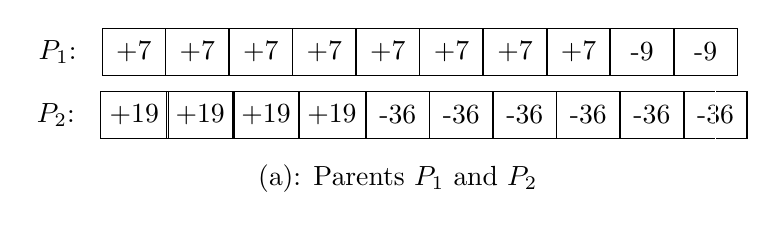
\begin{tikzpicture}
\tikzstyle{rec} = [rectangle, minimum width=0.8cm,minimum height=0.6cm, text
centered, draw=black]
	\node (gene11) [rec] {+7};
	\node (gene2) [rec] at ($(gene11.east)+(0.4cm,0)$)  {+7};
	\node (gene3) [rec] at ($(gene2.east)+(0.4cm,0)$)  {+7};
	\node (gene4) [rec] at ($(gene3.east)+(0.4cm,0)$)  {+7};
	\node (gene5) [rec] at ($(gene4.east)+(0.4cm,0)$)  {+7};
	\node (gene6) [rec] at ($(gene5.east)+(0.4cm,0)$)  {+7};
	\node (gene7) [rec] at ($(gene6.east)+(0.4cm,0)$)  {+7};
	\node (gene8) [rec] at ($(gene7.east)+(0.4cm,0)$)  {+7};
	\node (gene9) [rec] at ($(gene8.east)+(0.4cm,0)$)  {-9};
	\node (last) [rec] at ($(gene9.east)+(0.4cm,0)$)  {-9};
	\node[text width=1cm] at ($(gene11.west)+(-0.3cm,0)$) {$P_1$:};
	\node (gene1) [rec] at ($(gene11.east)+(-0.4cm,-0.8cm)$) {+19};
	\node (gene2) [rec] at ($(gene1.east)+(0.4cm,0)$)  {+19};
	\node (gene3) [rec] at ($(gene2.east)+(0.4cm,0)$)  {+19};
	\node (gene4) [rec] at ($(gene3.east)+(0.4cm,0)$)  {+19};
	\node (gene5) [rec] at ($(gene4.east)+(0.4cm,0)$)  {-36};
	\node (gene6) [rec] at ($(gene5.east)+(0.4cm,0)$)  {-36};
	\node (gene7) [rec] at ($(gene6.east)+(0.4cm,0)$)  {-36};
	\node (gene8) [rec] at ($(gene7.east)+(0.4cm,0)$)  {-36};
	\node (gene9) [rec] at ($(gene8.east)+(0.4cm,0)$)  {-36};
	\node (gene10) [rec] at ($(gene9.east)+(0.4cm,0)$)  {-36};
	\node[text width=1cm] at ($(gene1.west)+(-0.3cm,0)$) {$P_2$:};
	\draw[-,white] ($(gene10.north)$)-- ++(0,-1.5cm);
	\node (label1) at ($(gene5.south)+(0cm,-0.5cm)$) {(a): Parents $P_1$ and $P_2$};
\end{tikzpicture}

% offspring
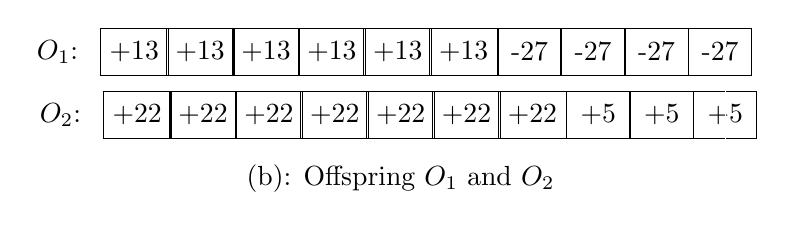
\begin{tikzpicture}
	\tikzstyle{rec} = [rectangle, minimum width=0.8cm,minimum height=0.6cm, text
	centered, draw=black]
	\node (gene11) [rec] {+13};
	\node (gene2) [rec] at ($(gene11.east)+(0.4cm,0)$)  {+13};
	\node (gene3) [rec] at ($(gene2.east)+(0.4cm,0)$)  {+13};
	\node (gene4) [rec] at ($(gene3.east)+(0.4cm,0)$)  {+13};
	\node (gene5) [rec] at ($(gene4.east)+(0.4cm,0)$)  {+13};
	\node (gene6) [rec] at ($(gene5.east)+(0.4cm,0)$)  {+13};
	\node (gene7) [rec] at ($(gene6.east)+(0.4cm,0)$)  {-27};
	\node (gene8) [rec] at ($(gene7.east)+(0.4cm,0)$)  {-27};
	\node (gene9) [rec] at ($(gene8.east)+(0.4cm,0)$)  {-27};
	\node (last) [rec] at ($(gene9.east)+(0.4cm,0)$)  {-27};
	\node[text width=1cm] at ($(gene11.west)+(-0.3cm,0)$) {$O_1$:};
	\node (gene1) [rec] at ($(gene11.east)+(-0.4cm,-0.8cm)$) {+22};
	\node (gene2) [rec] at ($(gene1.east)+(0.4cm,0)$)  {+22};
	\node (gene3) [rec] at ($(gene2.east)+(0.4cm,0)$)  {+22};
	\node (gene4) [rec] at ($(gene3.east)+(0.4cm,0)$)  {+22};
	\node (gene5) [rec] at ($(gene4.east)+(0.4cm,0)$)  {+22};
	\node (gene6) [rec] at ($(gene5.east)+(0.4cm,0)$)  {+22};
	\node (gene7) [rec] at ($(gene6.east)+(0.4cm,0)$)  {+22};
	\node (gene8) [rec] at ($(gene7.east)+(0.4cm,0)$)  {+5};
	\node (gene9) [rec] at ($(gene8.east)+(0.4cm,0)$)  {+5};
	\node (gene10) [rec] at ($(gene9.east)+(0.4cm,0)$)  {+5};
	\node[text width=1cm] at ($(gene1.west)+(-0.3cm,0)$) {$O_2$:};
	\draw[-,white] ($(gene10.north)$)-- ++(0,-1.5cm);
	\node (label1) at ($(gene5.south)+(0cm,-0.5cm)$) {(b): Offspring $O_1$ and $O_2$};
\end{tikzpicture}

%mutation
\begin{tikzpicture}
\tikzstyle{rec} = [rectangle, minimum width=0.8cm,minimum height=0.6cm, text
centered, draw=black]
	\tikzstyle{rec} = [rectangle, minimum width=0.8cm,minimum height=0.6cm, text
	centered, draw=black]
	%\draw[help lines](-3,-3) grid (4,4);
	\node (gene11) [rec] {+13};
	\node (gene2) [rec] at ($(gene11.east)+(0.4cm,0)$)  {+13};
	\node (gene3) [rec] at ($(gene2.east)+(0.4cm,0)$)  {+13};
	\node (gene4) [rec] at ($(gene3.east)+(0.4cm,0)$)  {$\cdots$};
	\node (gene5) [rec] at ($(gene4.east)+(0.4cm,0)$)  {+13};
	\node (gene6) [rec] at ($(gene5.east)+(0.4cm,0)$)  {+13};
	\node (gene7) [rec] at ($(gene6.east)+(0.4cm,0)$)  {-27};
	\node (gene8) [rec] at ($(gene7.east)+(0.4cm,0)$)  {$\cdots$};
	\node (gene9) [rec] at ($(gene8.east)+(0.4cm,0)$)  {-27};
	\node (last) [rec] at ($(gene9.east)+(0.4cm,0)$)  {-27};
	\draw[<->,thick] (gene11.south) .. controls +(1.8,-0.4) .. (gene6.south)
		node[pos=0.5] {11} ;
	\draw[<->,thick] (gene7.south) .. controls +(1.3,-0.4) .. (last.south)
		node[pos=0.5] {7};
	\node[text width=1cm] at ($(gene11.west)+(-0.3cm,0)$) {$O_1$:};

	\node (gene1) [rec] at ($(gene11.east)+(-0.4cm,-1.2cm)$) {+22};
	\node (gene2) [rec] at ($(gene1.east)+(0.4cm,0)$)  {+13};
	\node (gene3) [rec] at ($(gene2.east)+(0.4cm,0)$)  {+13};
	\node (gene4) [rec] at ($(gene3.east)+(0.4cm,0)$)  {$\cdots$};
	\node (gene5) [rec] at ($(gene4.east)+(0.4cm,0)$)  {+13};
	\node (gene6) [rec] at ($(gene5.east)+(0.4cm,0)$)  {+13};
	\node (gene7) [rec] at ($(gene6.east)+(0.4cm,0)$)  {-27};
	\node (gene8) [rec] at ($(gene7.east)+(0.4cm,0)$)  {$\cdots$};
	\node (gene9) [rec] at ($(gene8.east)+(0.4cm,0)$)  {-27};
	\node (last) [rec] at ($(gene9.east)+(0.4cm,0)$)  {-27};
	\draw[<->,thick] (gene1.south) .. controls +(1.8,-0.4) .. (gene6.south);
	\draw[<->,thick] (gene7.south) .. controls +(1.3,-0.4) .. (last.south);
	\node[text width=1cm] at ($(gene11.west)+(-0.3cm,0)$) {$O_1$:};
	\draw[-,white] ($(gene10.north)$)-- ++(0,-1.5cm);
	\node (label1) at ($(gene5.south)+(0cm,-0.5cm)$) {(b): Offspring $O_1$ and
		$O_2$ after mutation};
\end{tikzpicture}
\end{center}
\caption{GA Operators\label{GA:operator}}
\end{figure}

\begin{figure*}
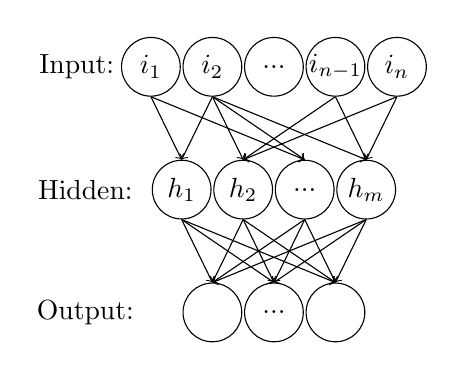
\begin{tikzpicture}
[ plain/.style={ draw=none, fill=none, }, remember picture, net/.style={ matrix of nodes, nodes={ draw, circle,
    inner sep=7.5pt
    },
  nodes in empty cells,
  column sep=-10.5pt,
  row sep=0.8cm
  }
]
%\draw[help lines] (-3cm,-6cm) grid (6cm,3cm);
\matrix[net] (mat)
{
              & |[plain]| &           & |[plain]|  &           & |[plain]| &           &  |[plain]|      &               \\
    |[plain]| &           & |[plain]| &            & |[plain]| &           & |[plain]| &                 & |[plain]|     \\ 
    |[plain]| & |[plain]| &           & |[plain]|  &           & |[plain]| & 	  	   &  |[plain]|      & |[plain]|     \\ 
  };

  \node at ($(mat-1-1.west)+(-16pt,0)$) {Input: };
  \node at ($(mat-2-2.west)+(-24pt,0)$) {Hidden:};
  \node at ($(mat-3-2.west)+(-24pt,0)$) {Output:};
  \node at (mat-1-1.base) {$i_1$};
  \node at (mat-1-3.base) {$i_2$};
  \node at (mat-1-5.base) {...};
  \node at (mat-1-7.base) {$i_{n-1}$};
  \node at (mat-1-9.base) {$i_{n}$};
  \node at (mat-2-2.base) {$h_1$};
  \node at (mat-2-4.base) {$h_2$};
  \node at (mat-2-6.base) {$...$};
  \node at (mat-2-8.base) {$h_{m}$};
  \node at (mat-3-5.base) {$...$};

 \foreach \a in {1,3}{
    \foreach \b in {2,6}{
        \draw[->] (mat-1-\a.south) -- (mat-2-\b.north);
     }
  }
 \foreach \a in {3,7,9}{
    \foreach \b in {4,8}{
        \draw[->] (mat-1-\a.south) -- (mat-2-\b.north);
     }
  }

 \foreach \c in {2,4,6,8}{
    \foreach \d in {3,5,7}{
 		\draw[->] (mat-2-\c.south) -- (mat-3-\d.north);
	}
 }
\end{tikzpicture}
\caption{Neural Network Model}
\end{figure*}



\begin{figure}
\centering
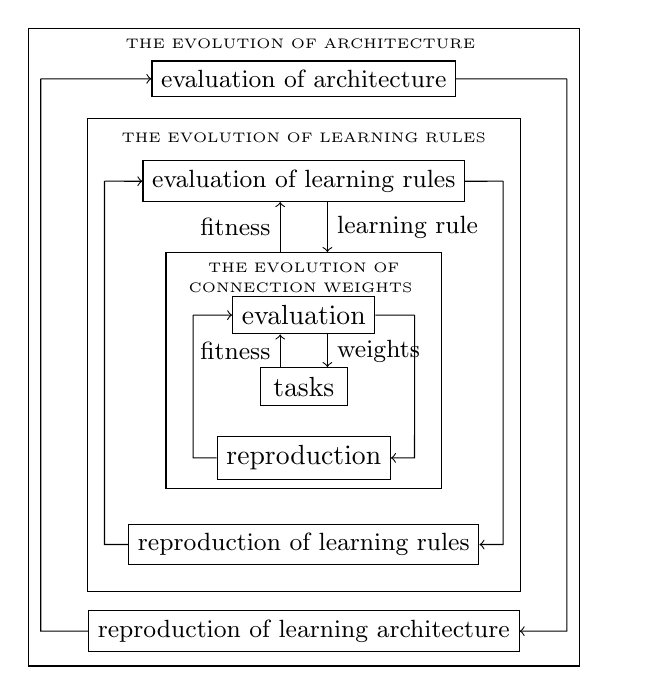
\begin{tikzpicture}
    %\draw[help lines] (-3cm,-6cm) grid (6cm, 6cm);
    \tikzstyle{block} = [rectangle, text centered, draw=black,
    minimum width=1.1cm, minimum height=0.4cm]
    % first level
    \node (evaluation-parent) [block, minimum width=2.4cm, minimum
        height=1.8cm,draw=white] {};
    \node (evaluation) [block] at ($(evaluation-parent.north)$) {evaluation};
    \node (reproduction) [block] at ($(evaluation-parent.south)$) {reproduction};
    \node (tasks) [block, minimum width=1.1cm, minimum height=0.4cm] {tasks};

    \draw[->] ($(evaluation.south)+(0.3cm,0cm)$) --
        ($(tasks.north)+(0.3cm,0cm)$) node[auto=left, pos=0.5] {\small weights}; 
    \draw[<-] ($(evaluation.south)+(-0.3cm,0cm)$) --
        ($(tasks.north)+(-0.3cm,0cm)$) node[auto=right, pos=0.5] {\small fitness}; 

    % get intersection
    \draw[white] (evaluation.west) coordinate (A) -- ++(-1.5cm,0) coordinate (B);
    \draw[white] (reproduction.west) -- ++(-0.3cm,0) coordinate (C) -- ++(0,4cm) coordinate
        (D);
    \draw[black] (reproduction.west) -- ++(-0.3cm,0) -- (intersection cs:
        first line={(A)--(B)}, second line={(C)--(D)}) coordinate (E);
    \draw[->] (E) -- (evaluation.west);

    \draw[white] (evaluation.east) coordinate (E) -- ++(2cm,0) coordinate (F);
    \draw[white] (reproduction.east) -- ++(0.3cm,0) coordinate (G) -- ++(0,4cm) coordinate
        (H);
    \draw[<-] (reproduction.east) -- ++(0.3cm,0) -- (intersection cs:
        first line={(E)--(F)}, second line={(G)--(H)}) coordinate (I);
    \draw (I) -- (evaluation.east);

    % second level
    \node (level2) [block,draw=black, minimum width=3.5cm, minimum height=3.0cm] at
        (0cm,0.2cm) {};
    \node [align=left] at ($(level2.north)+(0,-0.2cm)$) {\tiny THE EVOLUTION
        OF};
    \node [align=left] at ($(level2.north)+(0,-0.45cm)$) {\tiny CONNECTION
            WEIGHTS 
        };
    % third level
    \node (level3-assister) [block, draw=white, minimum width=5cm, minimum
		height=4.6cm] at
        (0, 0.3cm)  {};
    \node (evaluation) [block] at ($(level3-assister.north)$) {\small evaluation of
        learning rules};
    \node (reproduction) [block] at ($(level3-assister.south)$) {\small reproduction of
        learning rules};

    \draw[->] ($(evaluation.south)+(0.3cm,0cm)$) --
        ($(level2.north)+(0.3cm,0cm)$) node[auto=left, pos=0.5] {\small learning
        rule}; 
    \draw[<-] ($(evaluation.south)+(-0.3cm,0cm)$) --
        ($(level2.north)+(-0.3cm,0cm)$) node[auto=right, pos=0.5] {\small fitness}; 

    \draw[white] (evaluation.west) coordinate (A) -- ++(-1.3cm,0) coordinate (B);
    \draw[white] (reproduction.west) -- ++(-0.3cm,0) coordinate (C) -- ++(0,4cm) coordinate
        (D);
    \draw[black] (reproduction.west) -- ++(-0.3cm,0) -- (intersection cs:
        first line={(A)--(B)}, second line={(C)--(D)}) coordinate (E);
    \draw[->] (E) -- (evaluation.west);

    \draw[white] (evaluation.east) coordinate (E) -- ++(2cm,0) coordinate (F);
    \draw[white] (reproduction.east) -- ++(0.3cm,0) coordinate (G) -- ++(0,4cm) coordinate
        (H);
    \draw[<-] (reproduction.east) -- ++(0.3cm,0) -- (intersection cs:
        first line={(E)--(F)}, second line={(G)--(H)}) coordinate (I);
    \draw (I) -- (evaluation.east);
   % fourth level
    \node (level4) [block, draw=black, minimum width=5.5cm, minimum
        height=6.0cm] at
        (0, 0.4cm)  {};
    \node [align=left] at ($(level4.north)+(0,-0.25cm)$) {\tiny THE EVOLUTION
        OF LEARNING RULES};
    % level five
    \node (level5-assister) [block, draw=white, minimum width=6.4cm, minimum
        height=7.0cm] at
        (0, 0.4cm)  {};
    \node (evaluation) [block] at ($(level5-assister.north)$) {\small evaluation of
        architecture};
    \node (reproduction) [block] at ($(level5-assister.south)$) {\small reproduction of
        learning architecture};

    \draw[white] (evaluation.west) coordinate (A) -- ++(-1.5cm,0) coordinate (B);
    \draw[white] (reproduction.west) -- ++(-0.6cm,0) coordinate (C) -- ++(0,4cm) coordinate
        (D);
    \draw[black] (reproduction.west) -- ++(-0.6cm,0) -- (intersection cs:
        first line={(A)--(B)}, second line={(C)--(D)}) coordinate (E);
    \draw[->] (E) -- (evaluation.west);

    \draw[white] (evaluation.east) coordinate (E) -- ++(2cm,0) coordinate (F);
    \draw[white] (reproduction.east) -- ++(0.6cm,0) coordinate (G) -- ++(0,4cm) coordinate
        (H);
    \draw[<-] (reproduction.east) -- ++(0.6cm,0) -- (intersection cs:
        first line={(E)--(F)}, second line={(G)--(H)}) coordinate (I);
    \draw (I) -- (evaluation.east);
    % level 6
    \node (level6) [block, minimum width=7.0cm, minimum
        height=8.1cm] at
        (0, 0.5cm)  {};
    \node [align=left] at ($(level6.north)+(0,-0.2cm)$) {\tiny THE EVOLUTION OF
            ARCHITECTURE
        };
\end{tikzpicture}
\caption{Genetic algorithm and artificial neural network}
\end{figure}


\begin{figure*}
\centering
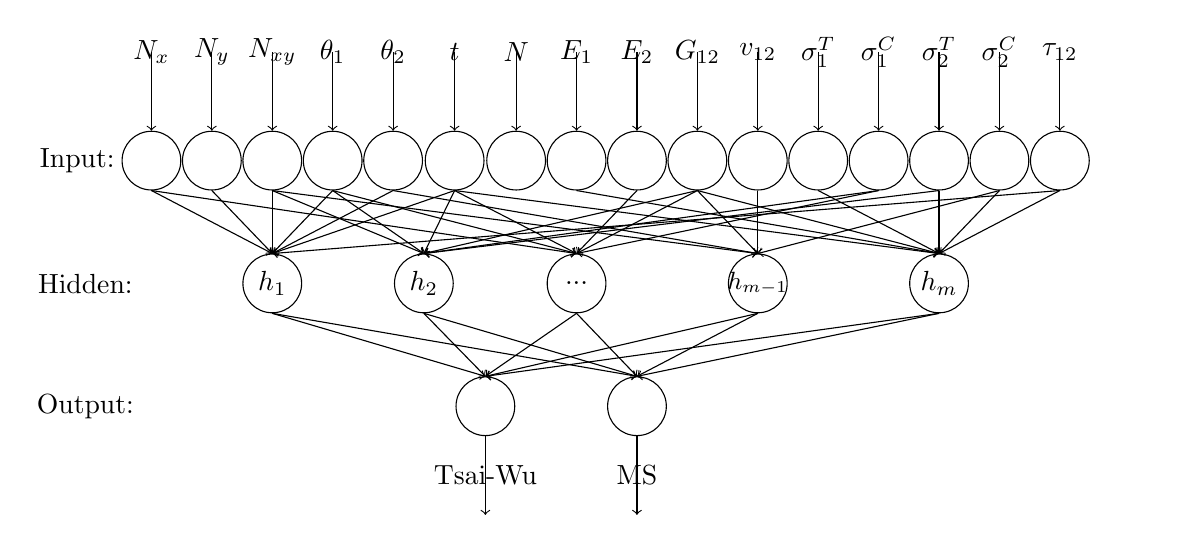
\begin{tikzpicture}
[ p/.style={ draw=none, fill=none, }, remember picture, 
  net/.style={ matrix of nodes, nodes={ draw, circle, inner sep=7.5pt },
  nodes in empty cells,
  column sep=-10.5pt,
  row sep=0.8cm
  }
]
%\draw[help lines] (-3cm,-6cm) grid (6cm,3cm);
\matrix[net] (mat)
{
	  & |[p]| &  & |[p]| &  & |[p]| &  & |[p]| &  & |[p]| &  & |[p]| &  & |[p]| &  & |[p]| &  &
	    |[p]| &  & |[p]| &  & |[p]| &  & |[p]| &  & |[p]| &  & |[p]| &  & |[p]| &  & |[p]|    \\
 |[p]| & |[p]| & |[p]| &  |[p]| &        & |[p]| & |[p]| & |[p]| &|[p]| &       & |[p]| &  |[p]| & |[p]| &
 |[p]| &       & |[p]| &  |[p]| &  |[p]| & |[p]| & |[p]| &       &|[p]| & |[p]| & |[p]| & |[p]|
	   & |[p]| &       &  |[p]| &  |[p]| & |[p]| & |[p]| & |[p]| &|[p]| \\ 
 |[p]| &  |[p]| & |[p]|  &  |[p]| & |[p]|  &  |[p]| &  |[p]| &  |[p]| & |[p]| & |[p]| & |[p]| &       & |[p]|
	   &  |[p]| & |[p]|  &  |[p]| &        &  |[p]| &  |[p]| &  |[p]| & |[p]| & |[p]| & |[p]| & |[p]| &     |[p]|
	   &  |[p]| & |[p]|  &  |[p]| & |[p]|  &  |[p]| &  |[p]| &  |[p]| \\ 
  };
  \draw[<-] (mat-1-1.north) --  ++(0,1) node {$N_x$};
  \draw[<-] (mat-1-3.north) --  ++(0,1) node {$N_y$};
  \draw[<-] (mat-1-5.north) --  ++(0,1) node {$N_{xy}$};
  \draw[<-] (mat-1-7.north) --  ++(0,1) node {$\theta_1$};
  \draw[<-] (mat-1-9.north) --  ++(0,1) node {$\theta_2$};
  \draw[<-] (mat-1-11.north) --  ++(0,1) node {$t$};
  \draw[<-] (mat-1-13.north) --  ++(0,1) node {$N$};
  \draw[<-] (mat-1-15.north) --  ++(0,1) node {$E_1$};
  \draw[<-] (mat-1-17.north) --  ++(0,1) node {$E_2$};
  \draw[<-] (mat-1-19.north) --  ++(0,1) node {$G_{12}$};
  \draw[<-] (mat-1-21.north) --  ++(0,1) node {$v_{12}$};
  \draw[<-] (mat-1-23.north) --  ++(0,1) node {$\sigma_1^T$};
  \draw[<-] (mat-1-25.north) --  ++(0,1) node {$\sigma_1^C$};
  \draw[<-] (mat-1-27.north) --  ++(0,1) node {$\sigma_2^T$};
  \draw[<-] (mat-1-29.north) --  ++(0,1) node {$\sigma_2^C$};
  \draw[<-] (mat-1-31.north) --  ++(0,1) node {$\tau_{12}$};
  \draw[->] (mat-3-12.south) --  ++(0,-1) node[pos=0.5, swap] {Tsai-Wu};
  \draw[->] (mat-3-17.south) --  ++(0,-1) node[pos=0.5, swap] {MS};
  \node at ($(mat-1-1.west)+(-16pt,0)$) {Input: };
  \node at ($(mat-2-2.west)+(-24pt,0)$) {Hidden:};
  \node at ($(mat-3-2.west)+(-24pt,0)$) {Output:};
  \node at (mat-2-5.base) {$h_1$};
  \node at (mat-2-10.base) {$h_2$};
  \node at (mat-2-15.base) {$...$};
  \node at (mat-2-21.base) {\small{$h_{m-1}$}};
  \node at (mat-2-27.base) {$h_{m}$};
 \foreach \a in {1,3,5,7,9,11,31}{
        \draw[->] (mat-1-\a.south) -- (mat-2-5.north);
     }
 \foreach \a in {5,7,11,19,25,27}{
        \draw[->] (mat-1-\a.south) -- (mat-2-10.north);
     }
 \foreach \a in {1,7,11,17,19,25}{
        \draw[->] (mat-1-\a.south) -- (mat-2-15.north);
     }
 \foreach \a in {5,9,19,21,29}{
        \draw[->] (mat-1-\a.south) -- (mat-2-21.north);
     }
 \foreach \a in {11,15,19,23,27,29,31}{
        \draw[->] (mat-1-\a.south) -- (mat-2-27.north);
     }
 \foreach \c in {5,10,15,21,27}{
    \foreach \d in {12,17}{
 		\draw[->] (mat-2-\c.south) -- (mat-3-\d.north);
	}
 }
\end{tikzpicture}
\caption{Neural Network Model}
\end{figure*}



The inputs of the neural network is consist of four parts: in-plane loading
$N_x$, $N_y$, and $N_{xy}$, design parameters of laminate, two distinct fiber
orientation angle $\theta_1$ and $\theta_2$, ply thickness $t$, total number of
plies $N$; five engineering constants of composite materials, $E_1$, $E_2$, ;
five strength parameters of a unidirectional lamina. There are two outputs in
the neural network, safety factors for MS theory and Tsai-Wu theory, respectively.

\begin{figure}
\centering
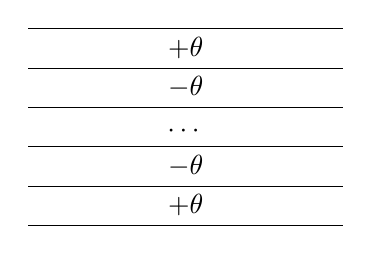
\begin{tikzpicture}
	\draw (0,0) -- (4,0);
	\draw (0,-0.5) -- (4,-0.5) node[midway, above] {$\mathit{+}\theta$};
	\draw (0,-1) -- (4,-1) node[midway, above] {$\mathit{-}\theta$} ;
	\draw (0,-1.5) -- (4,-1.5) node[midway, above] {$\cdots$};
	\draw (0,-2) -- (4,-2) node[midway, above] {$\mathit{-}\theta$};
	\draw (0,-2.5) -- (4,-2.5) node[midway, above] {$\mathit{+}\theta$};
\end{tikzpicture}
\caption{Model for Angle ply laminate}
\end{figure}






\section{Conclusion}
We review the use of genetic algorithms and artificial neural networks as an
alternative approach for calculating the strength ratio of an angle ply
laminate under in-plane loading, traditionally, which is obtained through CLT,
and corresponding failure theories, such as Maximum stress theory and Tsai-wu
failure theory. To obtain optimal architecture, we propose a two-layer ANN
framework and four levels of evolution on the design of ANN.  It was
demonstrated that ANN is an efficient and simple tool to compute the strength
ratio, instead of the complex analytical mathematical model. Our findings
underline the practical applicability of ANN on the analysis of composite
material.  



\section*{Acknowledgment}
The paper was supported by China Scholarship Council with
the code number 201806630112


\bibliographystyle{IEEEtran}
\bibliography{src/a6_reference}

\end{document}


